%  !TeX  root  =  user_guide.tex

\chapter{Первые шаги}\label{label_getstarted}

% when the revision of a section has been finalized,
% comment out the following line:
% \updatedisclaimer

В этом разделе даётся краткий обзор процесса установки \qg и пробных
данных, а также приводится пример сеанса работы с выводом растровых и векторных
слоёв.

\section{Установка}\label{label_installation}
\index{установка}

Процесс установки \qg очень прост. Пакеты для стандартной установки
доступны для MS Windows и Mac~OS\,X. Для разнообразных дистрибутивов
GNU/Linux существуют репозитории с пакетами в форматах rpm и deb. Самую
актуальную информацию по двоичным пакетам можно получить на сайте
\qg (\url{http://download.qgis.org}).

\minisec{Установка из исходного кода}

Инструкции по сборке \qg из исходного кода приведены в <<Руководстве
по программированию и компиляции>>, которое можно найти на странице
\url{http://www.qgis.org/en/documentation/manuals.html} или загрузить вместе
с исходным кодом \qg.

\minisec{Установка на внешний носитель}

В \qg добавлен параметр командной строки --configpath, который переопределяет
каталог, используемый для пользовательских настроек и расширений, по умолчанию
(например, ~/.qgis в Linux). Это позволяет выполнять установку \qg на сменный
носитель, например, USB-диск.

\section{Примеры данных}\label{label_sampledata}
\index{данные!примеры}

В данном руководстве приводятся приёмы работы, основанные на примерах данных
\qg.

\win Программа установки для Windows включает параметр, который позволяет
загрузить примеры данных \qg. При активации параметра данные будут загружены в папку
\filename{GIS DataBase} внутри папки \filename{Мои документы}
текущего пользователя. В дальнейшем, эту папку можно переместить в более
удобное место. Если во время первичной установки \qg флажок для загрузки
примеров данных не был отмечен, можно поступить следующим образом:
\begin{itemize}[label=--]
\item использовать уже имеющиеся данные;
\item загрузить примеры данных с сайта \qg по адресу \url{http://download.qgis.org}; или
\item при невозможности использовать один из вышеописанных способов "---
удалить \qg и переустановить её с выбраной опцией загрузки примеров данных.
\end{itemize}

\nix \osx Для GNU/Linux и Mac~OS\,X пока нет установочных пакетов
примеров данных, доступных в виде rpm, deb или dmg. Для использования
примеров данных необходимо загрузить файл \filename{QGIS\_sample\_data}
в виде архива ZIP или TAR по адресу
\url{http://download.osgeo.org/qgis/data/} и распаковать его. Набор
данных Alaska содержит все данные, которые используются в данном руководстве,
а также небольшую базу данных GRASS. В примере данных используется
проекция Alaska Albers Equal Area с футами в качестве единиц измерения.
Код EPSG (European Petroleum Survey Group) данной проекции "--- 2964.

\begin{verbatim}
PROJCS["Albers Equal Area",
    GEOGCS["NAD27",
        DATUM["North_American_Datum_1927",
            SPHEROID["Clarke 1866",6378206.4,294.978698213898,
                AUTHORITY["EPSG","7008"]],
            TOWGS84[-3,142,183,0,0,0,0],
            AUTHORITY["EPSG","6267"]],
        PRIMEM["Greenwich",0,
            AUTHORITY["EPSG","8901"]],
        UNIT["degree",0.0174532925199433,
            AUTHORITY["EPSG","9108"]],
        AUTHORITY["EPSG","4267"]],
    PROJECTION["Albers_Conic_Equal_Area"],
    PARAMETER["standard_parallel_1",55],
    PARAMETER["standard_parallel_2",65],
    PARAMETER["latitude_of_center",50],
    PARAMETER["longitude_of_center",-154],
    PARAMETER["false_easting",0],
    PARAMETER["false_northing",0],
    UNIT["us_survey_feet",0.3048006096012192]]
\end{verbatim}

Если вы собираетесь использовать \qg как графический интерфейс для
GRASS, на официальном веб-сайте ГИС GRASS
\url{http://grass.osgeo.org/download/data.php} можно найти примеры
<<областей>> GRASS (например, Spearfish или South Dakota).

\section{Пример сеанса работы}\label{samplesession}

Теперь, когда \qg установлена и доступны примеры данных, рассмотрим
простой пример сеанса работы в \qg. Мы выведем на экран растровый слой
почвенно-растительного покрова \\
(\filename{QGIS\_sample\_data/raster/landcover.img}) и векторный
слой озёр (\filename{QGIS\_sample\_data/gml/lakes.gml}).

\minisec{Запуск \qg}

\begin{itemize}[label=--]
\item \nix{Запустите \qg , набрав: \usertext{\qg} в командной строке, или
из меню Приложений, если вы установили пакет для вашего дистрибутива.}
\item \win{Запустите \qg , используя меню Пуск или ярлык на Рабочем столе,
или двойным щелчком на файле проекта \qg.}
\item \osx{Дважды щёлкните на значке \qg в папке Приложений.}
\end{itemize}

\begin{figure}[ht]
   \centering
   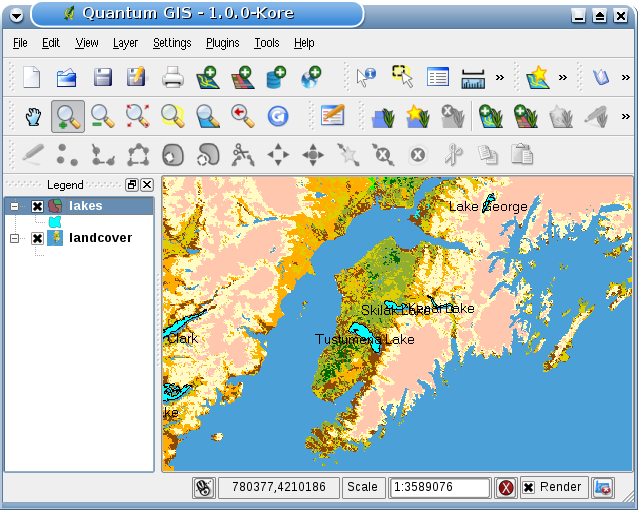
\includegraphics[clip=true, width=12cm]{simple_session}
   \caption{Пример сеанса работы \qg \wincaption}\label{fig:simple_session}
\end{figure}

\minisec{Загрузка пробных слоёв}

{\setlength{\baselineskip}{1.3\baselineskip}
\begin{enumerate}[itemsep=2pt]
\item Щёлкните на значке \toolbtntwo{mActionAddRasterLayer}{Добавить растровый слой}.
\item Откройте папку \filename{QGIS\_sample\_data/raster/}, выберите файл
формата ERDAS~Img \filename{landcover.img} и нажмите \button{Открыть}.
\item Если нужного файла нет в списке, проверьте, правильно ли указан
тип файлов в нижней части диалогового окна, в данном случае
<<Erdas Imagine Images (*.img, *.IMG)>>
\item Теперь щёлкните на значке \toolbtntwo{mActionAddOgrLayer}{Добавить векторный слой}.
\item \radiobuttonon{'Файл'} должен быть выбран как Тип источника в
новом окне \dialog{Добавить векторный слой}. Теперь нажмите \button{Обзор},
чтобы выбрать векторный слой.
\item Откройте папку \filename{QGIS\_sample\_data/gml/}, выберите <<GML>>
в выпадающем списке типа файлов, затем выберите файл GML (Geography Markup
Language) \filename{lakes.gml} и нажмите кнопку \button{Открыть}, затем в окне
\dialog{Добавить векторный слой} нажмите кнопку \button{Открыть}.
\item Немного увеличьте изображение территории с озерами.
\item Дважды щёлкните на слое \filename{lakes} в панели слоёв, чтобы открыть
окно \dialog{Свойства слоя}.
\item Перейдите на вкладку \tab{Стиль} и выберите синий в качестве
цвета заливки.
\item Перейдите на вкладку \tab{Подписи} и активируйте флажок
\checkbox{Включить подписи} для вывода подписей. Выберите значение
NAMES в выпадающем списке <<Поле, содержащее подпись>>.
\item Для улучшения читаемости подписей, можно добавить буфер белого
цвета вокруг них, включив флажок \checkbox{Буферизовать подписи} и
выбрав <<Размер буфера>> 3.
\item Нажмите \button{Применить}, убедитесь, что вас устраивает результат, и,
наконец, нажмите \button{ОК}.
\end{enumerate}
\par}
Как видите, в \qg очень просто вывести растровые и векторные слои. В следующих
главах вы узнаете больше о доступной функциональности, возможностях, настройках,
и о том, как всё это использовать.

\FloatBarrier
